\section{Theorie}

\subsection{Allgemeine Relaxation und die Anwendung in einem RC-Kreis }

\begin{flushleft}
    Das Phänomen bei dem ein System aus seinem Ausgangszustand, ohne Oszillation asymptotisch in denselben Zustand zurückkehrt, nennt man Relaxationserscheinung.
    Die Änderungsgeschwindigkeit der Größe A in einem Zeitpunkt $t$ ist proportional zur Abweichung der Größe A im Endzustand
\end{flushleft}

\begin{align}
    \frac{dA}{dt} = c \left[A(t)-A(\infty)\right].  \notag
    \intertext{Diese Gleichung lässt sich durch Umformen zu}
    A(t) = A(\infty) + \left[A(0) - A(\infty)\right] \label{1}
\end{align}

\begin{flushleft}
    lösen.
\end{flushleft}

\subsection{Entlade und Ladevorgang eines Kondensators im RC-Kreis}

\begin{align*}
    \intertext{Die Aufladung und Entladung eines Kondensators über einen Widerstand bilden Beispiele für Relaxationsvorgänge.}
    \intertext{\textbf{Entladevorgang:}}
    \intertext{Die Spannung des Kondensators $U_{\text{C}}$ wird durch die Ladung $Q$ und die Kapazität $C$ bestimmt}
    U_{\text{C}} = \frac{Q}{C}.
    \intertext{Durch den Widerstand $R$ fließt nach dem Ohmschen Gesetz ein Strom, welcher den Ladungsausgleich herbeiführt.}
    I = \frac{ U_{\text{C}}}{R}.
    \intertext{Die Ladung der Kondensatorplatten lässt durch}
    dQ = -I\,dt
\end{align*}
\begin{align}
    \intertext{beschreiben und führt mithilfe der restlichen Formeln zu dem zeitlichen Verlauf der Ladung des Kondensators, differentiell ausgedrückt}
    \frac{dQ}{dt} = \frac{1}{RC}\,Q(t). \label{3}
    \intertext{Dadurch, dass bei unendlich langer Entladung des Kondensators die Ladung gleich null ist und der Integration aus Formel (\ref{1}) wird die Lösung der DGL erhalten}
    Q\,(t) = Q(0) \cdot e^{\frac{-t}{RC}}\,. \label{4}
\end{align}

\begin{align*}
    \intertext{\textbf{Aufladevorgang:}}
    \intertext{Die Gleichung für die Aufladung eines Kondensators über einen Widerstand lässt sich durch die Randbedingungen}
    Q\,(0) = 0 
    \intertext{und}
    Q(\infty) = CU_{0}
    \intertext{herleiten. Dadurch setzt sich die DGL für den Aufladevorgang durch}
    Q(t) = CU_{0} (1 - e^{\frac{-t}{RC}})
    \intertext{zusammen. Der Ausdruck RC steht hierbei für die Zeitkonstante des Relaxationsvorganges und ist ein Maß für die Geschwindigkeit des Aufladevorganges.}
\end{align*}

\subsection{Relaxationsverhalten bei angelegter Spannung}

\begin{align}
    \intertext{Die Gleichung}
    U\,(t) = U_{0} \cdot \cos({\omega t})\notag
    \intertext{beschreibt allgemein die Wechselspannung. Die daraus enstehende Phasenverschiebung zwischen der eingehenden Spannung des Sinusgenerators
    und der ausgehenden Spannung des verzögerten Kondensators führt zu der Gleichung für die ausgehende Wechselspannung}
    U_{\text{C}}\,(t) = A\,(\omega)\, \cos(\omega t + \varphi(\omega)),\notag
    \intertext{wobei A die Kondensatorspannungsamplitude angibt.}
    \intertext{Mit Hilfe der Kirchhoffschen Gesetze, bezogen auf diese RC Schaltung,}
    U(t) = U_{\text{R}}(t) + U_{\text{C}}(t),\notag
    \intertext{dem zeitabhängigen Stromfluss}
    I(t) = \frac{dQ}{dt} = C\frac{dU_{\text{C}}}{dt},\notag
    \intertext{der frequenzabhängigen Phase}
    \phi (\omega) = \arctan (-\omega RC), \notag
    \intertext{sowie der Formel (\ref{3}) erhält man die Gleichung}
    A(\omega) = \frac{U_{0}}{\sqrt{1+\omega^2R^2C^2}}\,. \label{5}
    \intertext{Dies folgt dadurch, dass durch die Proportionalität der Phasenverschiebung zur Frequenz, bei niedrigen Frequenz die Phasenverschiebung gegen null geht.} \notag
\end{align}

\subsection{Die Phasenverschiebung}

\begin{flushleft}
    Die Phasenverschiebung lässt sich durch\\
    \vspace{0,2cm}
    \begin{equation}
        \varphi = \frac{a}{b} \cdot 2\pi \label{6}
    \end{equation}\\
    \vspace{0,4cm}
    berechnen, wobei a der Abstand beider Nullstellen zueinander und b die Wellenlänge in Bogenmaß beschreibt.
    Dabei geht $\varphi$  
\end{flushleft}

\begin{figure}     
    \centering
    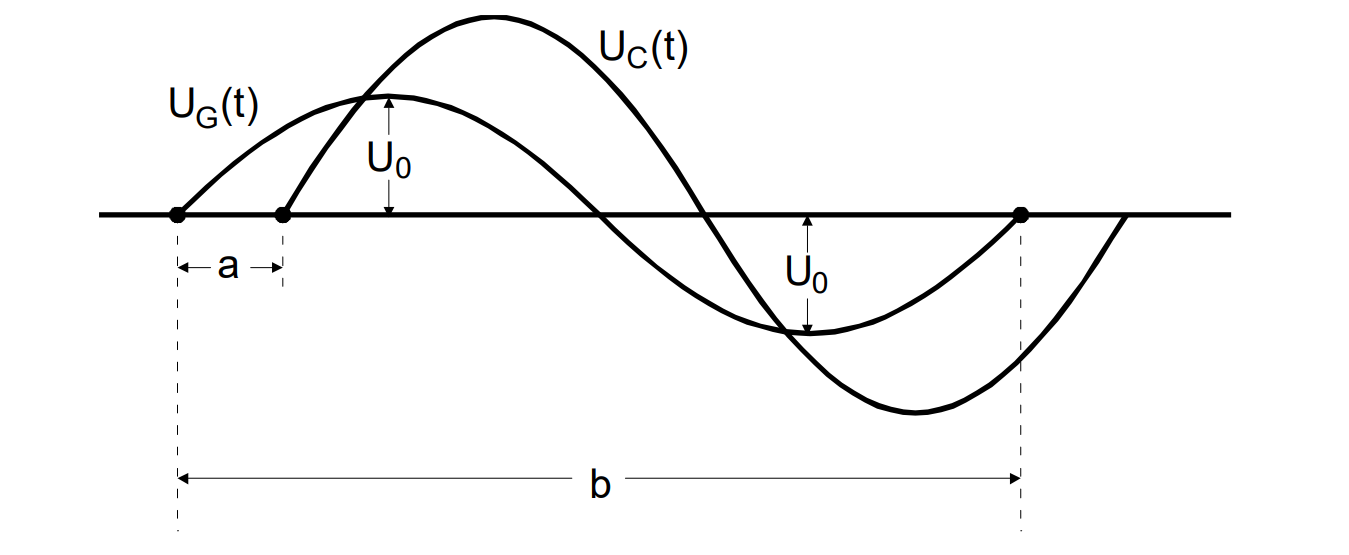
\includegraphics[width=125mm]{bilder/Abbildung2.png}
    \caption{Die Abbildung einer Phasenverschiebung \cite{a1}.\label{Abbildung1} }
\end{figure}

\subsection{Integrationsverhalten des RC-Kreises}

\begin{flushleft}
    Damit ein RC-Kreis als Integrator dienen kann, muss die Voraussetzung, dass $\omega >> \frac{1}{RC}$ ist, erfüllt sein.
    Durch die Formel 
\end{flushleft}

\begin{align*}
    U(t) = U_{\text{R}}(t) + U_{\text{C}}(t),
    \intertext{welche umgeschrieben wird zu}
    U(t) = R \cdot I(t) + U_{\text{C}}(t)
    \intertext{und einsetzen des zeitabhängigen Stromflusses, erhält man}
    U(t) = RC \cdot \frac{d U_{\text{C}}}{dt}+ U_{\text{C}}(t).
    \intertext{Durch die Vorraussetzung $\omega >> \frac{1}{RC}$, ist $|U_{\text{C}}|$ sehr viel kleiner als $|U_{\text{R}}|$ und $|U|$, wodurch näherungsweise geschrieben werden kann}
\end{align*}

\begin{equation}
    U_{\text{C}}(t) = \frac{1}{RC} \int_{0}^{t} U(t') \,dt'\,\,. \label{7}
\end{equation}